\scanpage{84}

\deleted{d'où $\Delta^{\unsure{\nu|v}}$ \deleted{\unsure{contr.|$A^*$}} $\inserted{\in A^{*}}$ donc $\Delta\in A^*$, et on va supposer}
\[
\deleted{\unsure{\text{\textcircled{h}}}\quad\boxed{\Delta\notin A^*}}
\]

Nous voulons prouver que $u_0$ est él. régulier de $A_0$, \deleted{si $A_0$ est intègre} i.e. qu'il n'est nul en aucune composante irréductible de $A_0$, ce qui résulte de ce qui précède.

\figure{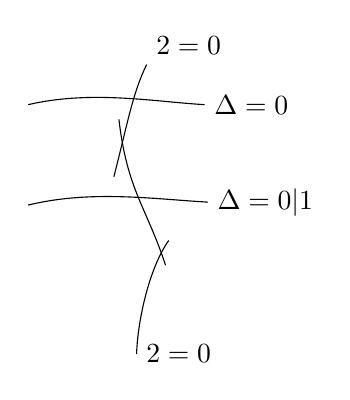
\begin{tikzpicture}[x=.8cm,y=.75cm]\draw (0,3.2) .. controls (1,3.45) and (2,3.25) .. (2.8,3.2) node[right] {$\Delta=0$};\draw (0,1.5) .. controls (1,1.76) and (2,1.6) .. (2.85,1.55) node[right] {$\Delta=\unsure{0|1}$};\draw (1.36,1.98) .. controls (1.58,2.9) and (1.66,3.4) .. (1.88,3.88) node[above right] {$2=0$};\draw (1.44,2.95) .. controls (1.57,1.75) and (1.88,1.46) .. (2.18,.48);\draw (2.23,.9) .. controls (1.93,.45) and (1.74,-.42) .. (1.72,-1.02) node[right] {$2=0$};\end{tikzpicture}}

Donc on trouve

\uline{Proposition} $A$ anneau, $\Delta\in A$. $A_0=A/2A$. On suppose, \inserted{$2$ $A$-régulier,} $A_0$ réduit, et intégral\textsuperscript{mt} clos dans son anneau total des fractions, $\Delta_0$ ($=\Delta$ mod $2$) \unsure{élém\textsuperscript{t}|élémt} régulier de $A_0$, \deleted{$A_0$}
$\{$ $\operatorname{Ker}(\operatorname{Pic}(A_{\Delta})\inserted{{}\to\operatorname{Pic}(A_{2\Delta})})=0$, $A_{\Delta}$ réduit et \deleted{\unsure{intégralt}} normal \unsure{clos|donc} \deleted{de $A_{2\Delta}$} en les pts de $V(A_0)$. $\}$
% slanted
\margin{il suffit que $A$ \unsure{noeth.|noeth|normal} et $A_0$ intègre}

\deleted{Pour que} \inserted{Conditions équivalentes :} \unsure{a)} il existe $b,c\in A$ avec
\[
b^2-4c=\Delta
\]

\deleted{\unsure{il f|il faut}} b) il existe une extension quadratique de $A$, \inserted{étale sur $A_{\Delta}$,} qui se réduit sur $A_{2\Delta}$ suivant l'extension étale $A_{2\Delta}[U]/(U^2-\Delta)$ [N.B. On \unsure{peut prendre|prendra} $A[T]/(T^2+bT+c)$]

b$'$) \deleted{\unsure{il}} existe une extension \inserted{finie} étale de $A_{\Delta}$ qui se réduit \deleted{\unsure{suivant}} \inserted{sur} $A_{2\Delta}$ suivant $A_{2\Delta}[U]/(U^2-\Delta)$
\margin{\uline{NB} il suffit qu'elle soit étale en les pts \unsure{minima|maxima|au dessus|maximaux} de \deleted{\unsure{$\operatorname{Spec}$}} $\operatorname{Spec} A_0$}
% archive sheet number: 83
